\documentclass[1p]{elsarticle_modified}
%\bibliographystyle{elsarticle-num}

%\usepackage[colorlinks]{hyperref}
%\usepackage{abbrmath_seonhwa} %\Abb, \Ascr, \Acal ,\Abf, \Afrak
\usepackage{amsfonts}
\usepackage{amssymb}
\usepackage{amsmath}
\usepackage{amsthm}
\usepackage{scalefnt}
\usepackage{amsbsy}
\usepackage{kotex}
\usepackage{caption}
\usepackage{subfig}
\usepackage{color}
\usepackage{graphicx}
\usepackage{xcolor} %% white, black, red, green, blue, cyan, magenta, yellow
\usepackage{float}
\usepackage{setspace}
\usepackage{hyperref}

\usepackage{tikz}
\usetikzlibrary{arrows}

\usepackage{multirow}
\usepackage{array} % fixed length table
\usepackage{hhline}

%%%%%%%%%%%%%%%%%%%%%
\makeatletter
\renewcommand*\env@matrix[1][\arraystretch]{%
	\edef\arraystretch{#1}%
	\hskip -\arraycolsep
	\let\@ifnextchar\new@ifnextchar
	\array{*\c@MaxMatrixCols c}}
\makeatother %https://tex.stackexchange.com/questions/14071/how-can-i-increase-the-line-spacing-in-a-matrix
%%%%%%%%%%%%%%%

\usepackage[normalem]{ulem}

\newcommand{\msout}[1]{\ifmmode\text{\sout{\ensuremath{#1}}}\else\sout{#1}\fi}
%SOURCE: \msout is \stkout macro in https://tex.stackexchange.com/questions/20609/strikeout-in-math-mode

\newcommand{\cancel}[1]{
	\ifmmode
	{\color{red}\msout{#1}}
	\else
	{\color{red}\sout{#1}}
	\fi
}

\newcommand{\add}[1]{
	{\color{blue}\uwave{#1}}
}

\newcommand{\replace}[2]{
	\ifmmode
	{\color{red}\msout{#1}}{\color{blue}\uwave{#2}}
	\else
	{\color{red}\sout{#1}}{\color{blue}\uwave{#2}}
	\fi
}

\newcommand{\Sol}{\mathcal{S}} %segment
\newcommand{\D}{D} %diagram
\newcommand{\A}{\mathcal{A}} %arc


%%%%%%%%%%%%%%%%%%%%%%%%%%%%%5 test

\def\sl{\operatorname{\textup{SL}}(2,\Cbb)}
\def\psl{\operatorname{\textup{PSL}}(2,\Cbb)}
\def\quan{\mkern 1mu \triangleright \mkern 1mu}

\theoremstyle{definition}
\newtheorem{thm}{Theorem}[section]
\newtheorem{prop}[thm]{Proposition}
\newtheorem{lem}[thm]{Lemma}
\newtheorem{ques}[thm]{Question}
\newtheorem{cor}[thm]{Corollary}
\newtheorem{defn}[thm]{Definition}
\newtheorem{exam}[thm]{Example}
\newtheorem{rmk}[thm]{Remark}
\newtheorem{alg}[thm]{Algorithm}

\newcommand{\I}{\sqrt{-1}}
\begin{document}

%\begin{frontmatter}
%
%\title{Boundary parabolic representations of knots up to 8 crossings}
%
%%% Group authors per affiliation:
%\author{Yunhi Cho} 
%\address{Department of Mathematics, University of Seoul, Seoul, Korea}
%\ead{yhcho@uos.ac.kr}
%
%
%\author{Seonhwa Kim} %\fnref{s_kim}}
%\address{Center for Geometry and Physics, Institute for Basic Science, Pohang, 37673, Korea}
%\ead{ryeona17@ibs.re.kr}
%
%\author{Hyuk Kim}
%\address{Department of Mathematical Sciences, Seoul National University, Seoul 08826, Korea}
%\ead{hyukkim@snu.ac.kr}
%
%\author{Seokbeom Yoon}
%\address{Department of Mathematical Sciences, Seoul National University, Seoul, 08826,  Korea}
%\ead{sbyoon15@snu.ac.kr}
%
%\begin{abstract}
%We find all boundary parabolic representation of knots up to 8 crossings.
%
%\end{abstract}
%\begin{keyword}
%    \MSC[2010] 57M25 
%\end{keyword}
%
%\end{frontmatter}

%\linenumbers
%\tableofcontents
%
\newcommand\colored[1]{\textcolor{white}{\rule[-0.35ex]{0.8em}{1.4ex}}\kern-0.8em\color{red} #1}%
%\newcommand\colored[1]{\textcolor{white}{ #1}\kern-2.17ex	\textcolor{white}{ #1}\kern-1.81ex	\textcolor{white}{ #1}\kern-2.15ex\color{red}#1	}

{\Large $\underline{12a_{0232}~(K12a_{0232})}$}

\setlength{\tabcolsep}{10pt}
\renewcommand{\arraystretch}{1.6}
\vspace{1cm}\begin{tabular}{m{100pt}>{\centering\arraybackslash}m{274pt}}
\multirow{5}{120pt}{
	\centering
	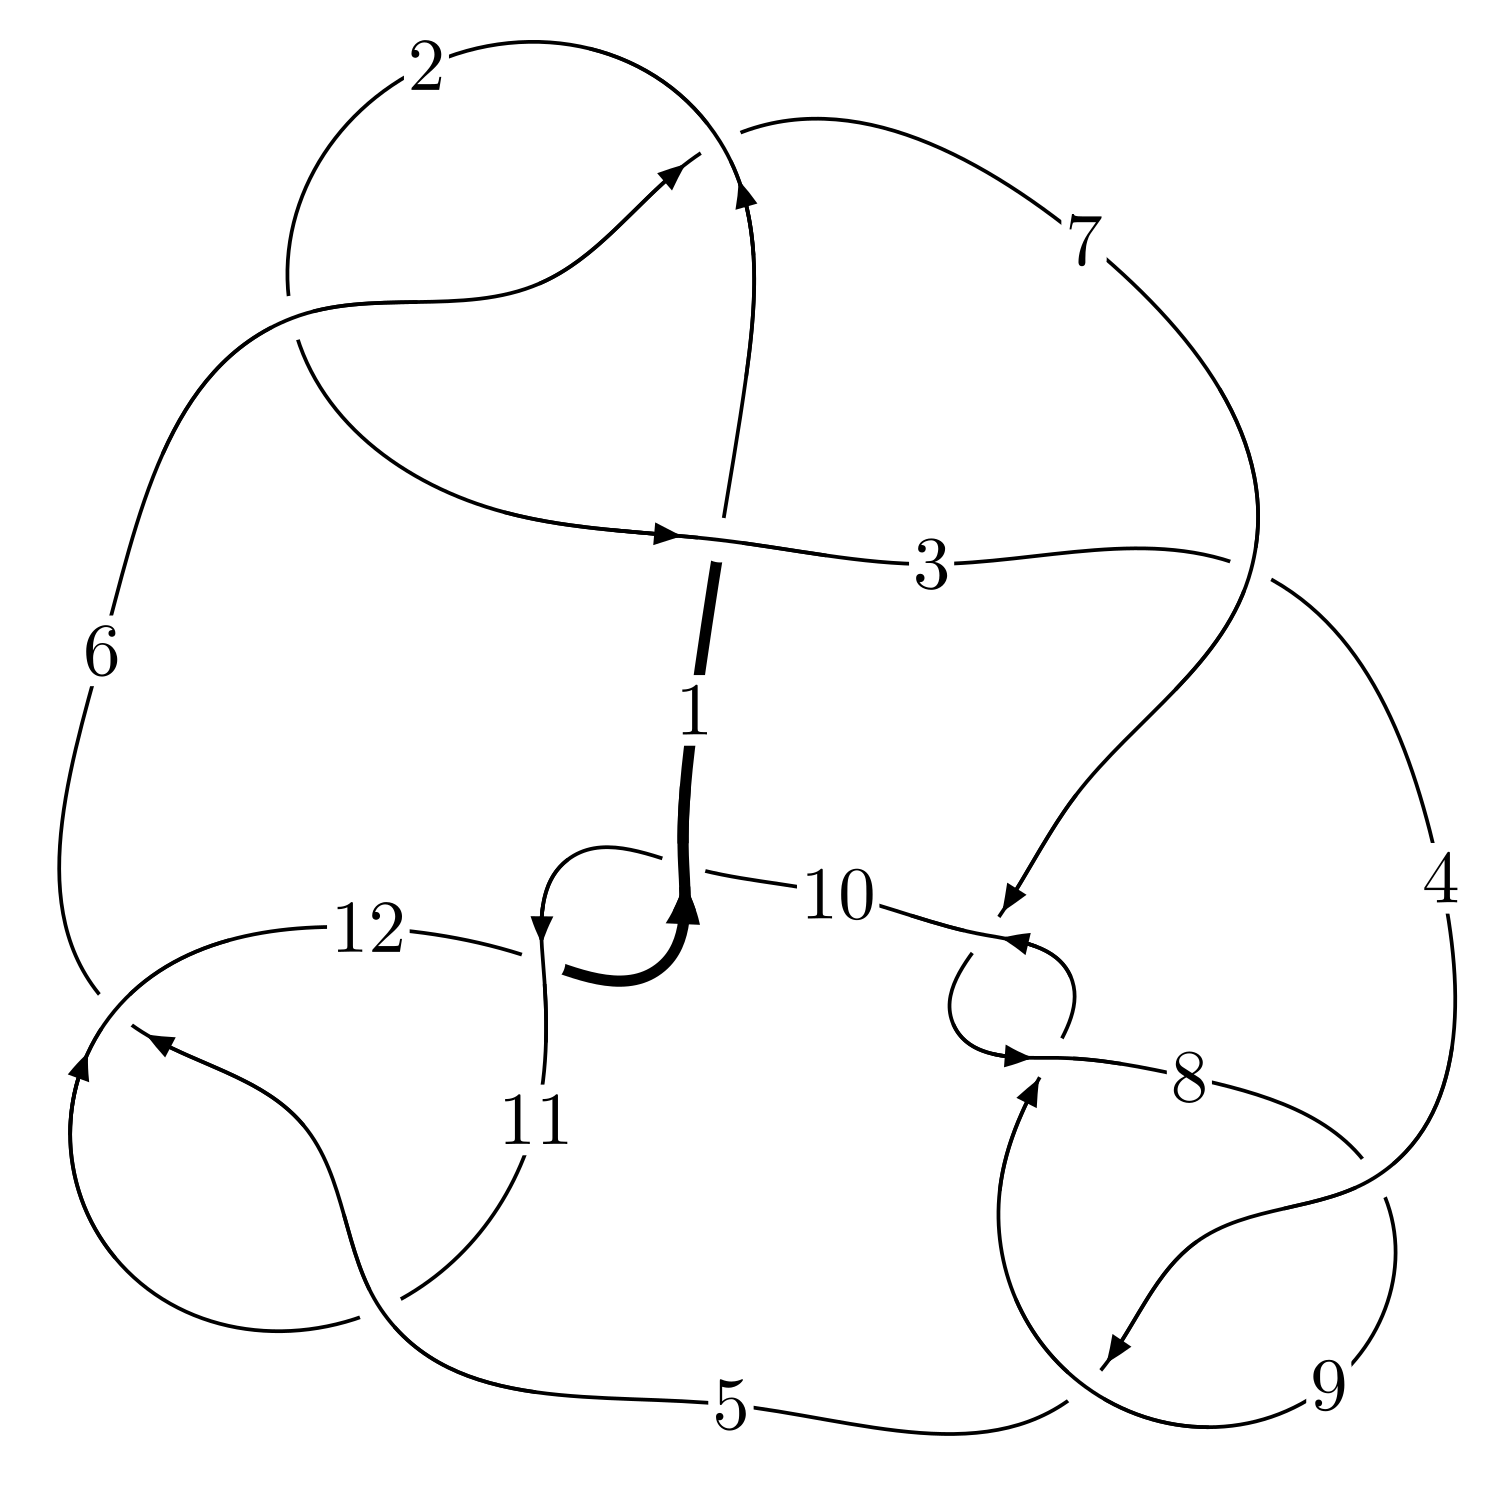
\includegraphics[width=112pt]{../../../GIT/diagram.site/Diagrams/png/1033_12a_0232.png}\\
\ \ \ A knot diagram\footnotemark}&
\allowdisplaybreaks
\textbf{Linearized knot diagam} \\
\cline{2-2}
 &
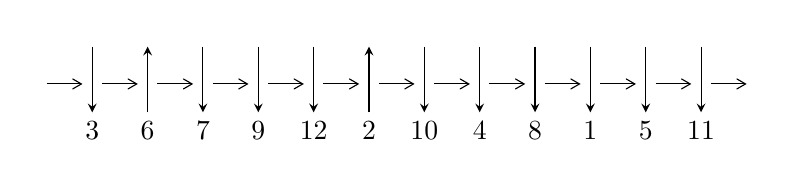
\begin{tikzpicture}[x=20pt, y=17pt]
	% nodes
	\node (C0) at (0, 0) {};
	\node (C1) at (1, 0) {};
	\node (C1U) at (1, +1) {};
	\node (C1D) at (1, -1) {3};

	\node (C2) at (2, 0) {};
	\node (C2U) at (2, +1) {};
	\node (C2D) at (2, -1) {6};

	\node (C3) at (3, 0) {};
	\node (C3U) at (3, +1) {};
	\node (C3D) at (3, -1) {7};

	\node (C4) at (4, 0) {};
	\node (C4U) at (4, +1) {};
	\node (C4D) at (4, -1) {9};

	\node (C5) at (5, 0) {};
	\node (C5U) at (5, +1) {};
	\node (C5D) at (5, -1) {12};

	\node (C6) at (6, 0) {};
	\node (C6U) at (6, +1) {};
	\node (C6D) at (6, -1) {2};

	\node (C7) at (7, 0) {};
	\node (C7U) at (7, +1) {};
	\node (C7D) at (7, -1) {10};

	\node (C8) at (8, 0) {};
	\node (C8U) at (8, +1) {};
	\node (C8D) at (8, -1) {4};

	\node (C9) at (9, 0) {};
	\node (C9U) at (9, +1) {};
	\node (C9D) at (9, -1) {8};

	\node (C10) at (10, 0) {};
	\node (C10U) at (10, +1) {};
	\node (C10D) at (10, -1) {1};

	\node (C11) at (11, 0) {};
	\node (C11U) at (11, +1) {};
	\node (C11D) at (11, -1) {5};

	\node (C12) at (12, 0) {};
	\node (C12U) at (12, +1) {};
	\node (C12D) at (12, -1) {11};
	\node (C13) at (13, 0) {};

	% arrows
	\draw[->,>={angle 60}]
	(C0) edge (C1) (C1) edge (C2) (C2) edge (C3) (C3) edge (C4) (C4) edge (C5) (C5) edge (C6) (C6) edge (C7) (C7) edge (C8) (C8) edge (C9) (C9) edge (C10) (C10) edge (C11) (C11) edge (C12) (C12) edge (C13) ;	\draw[->,>=stealth]
	(C1U) edge (C1D) (C2D) edge (C2U) (C3U) edge (C3D) (C4U) edge (C4D) (C5U) edge (C5D) (C6D) edge (C6U) (C7U) edge (C7D) (C8U) edge (C8D) (C9U) edge (C9D) (C10U) edge (C10D) (C11U) edge (C11D) (C12U) edge (C12D) ;
	\end{tikzpicture} \\
\hhline{~~} \\& 
\textbf{Solving Sequence} \\ \cline{2-2} 
 &
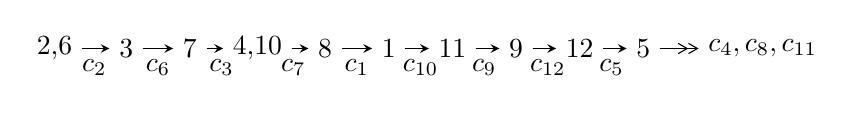
\begin{tikzpicture}[x=23pt, y=7pt]
	% node
	\node (A0) at (-1/8, 0) {2,6};
	\node (A1) at (1, 0) {3};
	\node (A2) at (2, 0) {7};
	\node (A3) at (49/16, 0) {4,10};
	\node (A4) at (33/8, 0) {8};
	\node (A5) at (41/8, 0) {1};
	\node (A6) at (49/8, 0) {11};
	\node (A7) at (57/8, 0) {9};
	\node (A8) at (65/8, 0) {12};
	\node (A9) at (73/8, 0) {5};
	\node (C1) at (1/2, -1) {$c_{2}$};
	\node (C2) at (3/2, -1) {$c_{6}$};
	\node (C3) at (5/2, -1) {$c_{3}$};
	\node (C4) at (29/8, -1) {$c_{7}$};
	\node (C5) at (37/8, -1) {$c_{1}$};
	\node (C6) at (45/8, -1) {$c_{10}$};
	\node (C7) at (53/8, -1) {$c_{9}$};
	\node (C8) at (61/8, -1) {$c_{12}$};
	\node (C9) at (69/8, -1) {$c_{5}$};
	\node (A10) at (11, 0) {$c_{4},c_{8},c_{11}$};

	% edge
	\draw[->,>=stealth]	
	(A0) edge (A1) (A1) edge (A2) (A2) edge (A3) (A3) edge (A4) (A4) edge (A5) (A5) edge (A6) (A6) edge (A7) (A7) edge (A8) (A8) edge (A9) ;
	\draw[->>,>={angle 60}]	
	(A9) edge (A10);
\end{tikzpicture} \\ 

\end{tabular} \\

\footnotetext{
The image of knot diagram is generated by the software ``\textbf{Draw programme}" developed by Andrew Bartholomew(\url{http://www.layer8.co.uk/maths/draw/index.htm\#Running-draw}), where we modified some parts for our purpose(\url{https://github.com/CATsTAILs/LinksPainter}).
}\phantom \\ \newline 
\centering \textbf{Ideals for irreducible components\footnotemark of $X_{\text{par}}$} 
 
\begin{align*}
I^u_{1}&=\langle 
-3 u^{23}-7 u^{22}+\cdots+4 b-22,\;u^{23}+15 u^{22}+\cdots+8 a-66,\;u^{24}+5 u^{23}+\cdots-12 u-4\rangle \\
I^u_{2}&=\langle 
- u^{37}+2 u^{36}+\cdots+2 b-1,\;- u^{37} a+3 u^{37}+\cdots+a-6,\;u^{38}-2 u^{37}+\cdots-2 u+1\rangle \\
I^u_{3}&=\langle 
- a u+b- a,\;a^2+a+1,\;u^2+1\rangle \\
I^u_{4}&=\langle 
a u+b- a+u,\;a^2+a+1,\;u^2+1\rangle \\
\\
\end{align*}
\raggedright * 4 irreducible components of $\dim_{\mathbb{C}}=0$, with total 108 representations.\\
\footnotetext{All coefficients of polynomials are rational numbers. But the coefficients are sometimes approximated in decimal forms when there is not enough margin.}
\newpage
\renewcommand{\arraystretch}{1}
\centering \section*{I. $I^u_{1}= \langle -3 u^{23}-7 u^{22}+\cdots+4 b-22,\;u^{23}+15 u^{22}+\cdots+8 a-66,\;u^{24}+5 u^{23}+\cdots-12 u-4 \rangle$}
\flushleft \textbf{(i) Arc colorings}\\
\begin{tabular}{m{7pt} m{180pt} m{7pt} m{180pt} }
\flushright $a_{2}=$&$\begin{pmatrix}1\\0\end{pmatrix}$ \\
\flushright $a_{6}=$&$\begin{pmatrix}0\\u\end{pmatrix}$ \\
\flushright $a_{3}=$&$\begin{pmatrix}1\\- u^2\end{pmatrix}$ \\
\flushright $a_{7}=$&$\begin{pmatrix}u\\u\end{pmatrix}$ \\
\flushright $a_{4}=$&$\begin{pmatrix}u^4+u^2+1\\u^4\end{pmatrix}$ \\
\flushright $a_{10}=$&$\begin{pmatrix}-0.125000 u^{23}-1.87500 u^{22}+\cdots+13.1250 u+8.25000\\\frac{3}{4} u^{23}+\frac{7}{4} u^{22}+\cdots+\frac{35}{4} u+\frac{11}{2}\end{pmatrix}$ \\
\flushright $a_{8}=$&$\begin{pmatrix}-\frac{1}{8} u^{23}-\frac{3}{8} u^{22}+\cdots+\frac{13}{8} u+\frac{3}{4}\\\frac{1}{4} u^{23}+\frac{5}{4} u^{22}+\cdots-\frac{3}{4} u-\frac{1}{2}\end{pmatrix}$ \\
\flushright $a_{1}=$&$\begin{pmatrix}u^2+1\\- u^4\end{pmatrix}$ \\
\flushright $a_{11}=$&$\begin{pmatrix}-\frac{3}{8} u^{23}-\frac{13}{8} u^{22}+\cdots+\frac{67}{8} u+\frac{19}{4}\\\frac{7}{4} u^{23}+\frac{29}{4} u^{22}+\cdots-\frac{21}{4} u-\frac{1}{2}\end{pmatrix}$ \\
\flushright $a_{9}=$&$\begin{pmatrix}-\frac{3}{8} u^{23}-\frac{9}{8} u^{22}+\cdots+\frac{35}{8} u+\frac{13}{4}\\\frac{3}{4} u^{23}+\frac{15}{4} u^{22}+\cdots-\frac{11}{4} u-\frac{1}{2}\end{pmatrix}$ \\
\flushright $a_{12}=$&$\begin{pmatrix}-\frac{1}{8} u^{23}-\frac{3}{8} u^{22}+\cdots+\frac{13}{8} u+\frac{7}{4}\\\frac{3}{4} u^{23}+\frac{13}{4} u^{22}+\cdots-\frac{17}{4} u-\frac{3}{2}\end{pmatrix}$ \\
\flushright $a_{5}=$&$\begin{pmatrix}\frac{7}{8} u^{23}+\frac{29}{8} u^{22}+\cdots-\frac{35}{8} u-\frac{11}{4}\\\frac{3}{4} u^{23}+\frac{7}{4} u^{22}+\cdots+\frac{35}{4} u+\frac{11}{2}\end{pmatrix}$\\&\end{tabular}
\flushleft \textbf{(ii) Obstruction class $= -1$}\\~\\
\flushleft \textbf{(iii) Cusp Shapes $= 11 u^{23}+55 u^{22}+202 u^{21}+511 u^{20}+1091 u^{19}+1935 u^{18}+3107 u^{17}+4507 u^{16}+6140 u^{15}+7797 u^{14}+9280 u^{13}+10305 u^{12}+10665 u^{11}+10334 u^{10}+9374 u^9+7922 u^8+6201 u^7+4343 u^6+2630 u^5+1231 u^4+311 u^3-76 u^2-124 u-58$}\\~\\
\newpage\renewcommand{\arraystretch}{1}
\flushleft \textbf{(iv) u-Polynomials at the component}\newline \\
\begin{tabular}{m{50pt}|m{274pt}}
Crossings & \hspace{64pt}u-Polynomials at each crossing \\
\hline $$\begin{aligned}c_{1}\end{aligned}$$&$\begin{aligned}
&u^{24}+13 u^{23}+\cdots-56 u+16
\end{aligned}$\\
\hline $$\begin{aligned}c_{2},c_{6}\end{aligned}$$&$\begin{aligned}
&u^{24}-5 u^{23}+\cdots+12 u-4
\end{aligned}$\\
\hline $$\begin{aligned}c_{3}\end{aligned}$$&$\begin{aligned}
&u^{24}+5 u^{23}+\cdots-256 u-64
\end{aligned}$\\
\hline $$\begin{aligned}c_{4},c_{5},c_{8}\\c_{11}\end{aligned}$$&$\begin{aligned}
&u^{24}-4 u^{22}+\cdots-2 u-1
\end{aligned}$\\
\hline $$\begin{aligned}c_{7},c_{9},c_{10}\\c_{12}\end{aligned}$$&$\begin{aligned}
&u^{24}+8 u^{23}+\cdots+4 u+1
\end{aligned}$\\
\hline
\end{tabular}\\~\\
\newpage\renewcommand{\arraystretch}{1}
\flushleft \textbf{(v) Riley Polynomials at the component}\newline \\
\begin{tabular}{m{50pt}|m{274pt}}
Crossings & \hspace{64pt}Riley Polynomials at each crossing \\
\hline $$\begin{aligned}c_{1}\end{aligned}$$&$\begin{aligned}
&y^{24}-3 y^{23}+\cdots-11552 y+256
\end{aligned}$\\
\hline $$\begin{aligned}c_{2},c_{6}\end{aligned}$$&$\begin{aligned}
&y^{24}+13 y^{23}+\cdots-56 y+16
\end{aligned}$\\
\hline $$\begin{aligned}c_{3}\end{aligned}$$&$\begin{aligned}
&y^{24}-7 y^{23}+\cdots-40960 y+4096
\end{aligned}$\\
\hline $$\begin{aligned}c_{4},c_{5},c_{8}\\c_{11}\end{aligned}$$&$\begin{aligned}
&y^{24}-8 y^{23}+\cdots-4 y+1
\end{aligned}$\\
\hline $$\begin{aligned}c_{7},c_{9},c_{10}\\c_{12}\end{aligned}$$&$\begin{aligned}
&y^{24}+20 y^{23}+\cdots+4 y+1
\end{aligned}$\\
\hline
\end{tabular}\\~\\
\newpage\flushleft \textbf{(vi) Complex Volumes and Cusp Shapes}
$$\begin{array}{c|c|c}  
\text{Solutions to }I^u_{1}& \I (\text{vol} + \sqrt{-1}CS) & \text{Cusp shape}\\
 \hline 
\begin{aligned}
u &= \phantom{-}0.257222 + 1.017220 I \\
a &= \phantom{-}0.401654 - 0.008767 I \\
b &= \phantom{-}0.272209 - 0.624992 I\end{aligned}
 & -3.50051 + 2.57930 I & -16.8117 - 4.7598 I \\ \hline\begin{aligned}
u &= \phantom{-}0.257222 - 1.017220 I \\
a &= \phantom{-}0.401654 + 0.008767 I \\
b &= \phantom{-}0.272209 + 0.624992 I\end{aligned}
 & -3.50051 - 2.57930 I & -16.8117 + 4.7598 I \\ \hline\begin{aligned}
u &= -0.908792 + 0.262544 I \\
a &= \phantom{-}1.44352 - 1.19871 I \\
b &= \phantom{-}0.476457 + 0.127868 I\end{aligned}
 & \phantom{-}3.72106 + 11.69860 I & -5.36042 - 8.05318 I \\ \hline\begin{aligned}
u &= -0.908792 - 0.262544 I \\
a &= \phantom{-}1.44352 + 1.19871 I \\
b &= \phantom{-}0.476457 - 0.127868 I\end{aligned}
 & \phantom{-}3.72106 - 11.69860 I & -5.36042 + 8.05318 I \\ \hline\begin{aligned}
u &= \phantom{-}0.769198 + 0.739991 I \\
a &= -0.486482 + 0.038089 I \\
b &= \phantom{-}0.467190 + 0.882825 I\end{aligned}
 & \phantom{-}7.88027 - 3.10260 I & -2.08649 + 2.69746 I \\ \hline\begin{aligned}
u &= \phantom{-}0.769198 - 0.739991 I \\
a &= -0.486482 - 0.038089 I \\
b &= \phantom{-}0.467190 - 0.882825 I\end{aligned}
 & \phantom{-}7.88027 + 3.10260 I & -2.08649 - 2.69746 I \\ \hline\begin{aligned}
u &= -0.848943 + 0.362352 I \\
a &= -1.20123 + 1.01267 I \\
b &= -0.567849 - 0.040943 I\end{aligned}
 & \phantom{-}5.70577 + 0.22260 I & -1.77984 + 2.03296 I \\ \hline\begin{aligned}
u &= -0.848943 - 0.362352 I \\
a &= -1.20123 - 1.01267 I \\
b &= -0.567849 + 0.040943 I\end{aligned}
 & \phantom{-}5.70577 - 0.22260 I & -1.77984 - 2.03296 I \\ \hline\begin{aligned}
u &= -0.292804 + 0.863918 I \\
a &= -0.320360 + 0.625045 I \\
b &= -0.081672 + 0.710622 I\end{aligned}
 & -0.53022 - 1.37947 I & -5.11379 + 4.42535 I \\ \hline\begin{aligned}
u &= -0.292804 - 0.863918 I \\
a &= -0.320360 - 0.625045 I \\
b &= -0.081672 - 0.710622 I\end{aligned}
 & -0.53022 + 1.37947 I & -5.11379 - 4.42535 I\\
 \hline 
 \end{array}$$\newpage$$\begin{array}{c|c|c}  
\text{Solutions to }I^u_{1}& \I (\text{vol} + \sqrt{-1}CS) & \text{Cusp shape}\\
 \hline 
\begin{aligned}
u &= \phantom{-}0.736879 + 0.861025 I \\
a &= \phantom{-}0.481995 - 0.036451 I \\
b &= -0.337196 - 1.007010 I\end{aligned}
 & \phantom{-}7.52630 + 8.69544 I & -3.16830 - 8.31175 I \\ \hline\begin{aligned}
u &= \phantom{-}0.736879 - 0.861025 I \\
a &= \phantom{-}0.481995 + 0.036451 I \\
b &= -0.337196 + 1.007010 I\end{aligned}
 & \phantom{-}7.52630 - 8.69544 I & -3.16830 + 8.31175 I \\ \hline\begin{aligned}
u &= -0.741563\phantom{ +0.000000I} \\
a &= \phantom{-}1.82111\phantom{ +0.000000I} \\
b &= \phantom{-}0.349010\phantom{ +0.000000I}\end{aligned}
 & -5.65295\phantom{ +0.000000I} & -15.3580\phantom{ +0.000000I} \\ \hline\begin{aligned}
u &= -0.441869 + 1.180010 I \\
a &= -0.07853 - 1.44892 I \\
b &= -0.32749 - 2.36407 I\end{aligned}
 & -9.05396 - 4.24780 I & -18.5113 + 3.9565 I \\ \hline\begin{aligned}
u &= -0.441869 - 1.180010 I \\
a &= -0.07853 + 1.44892 I \\
b &= -0.32749 + 2.36407 I\end{aligned}
 & -9.05396 + 4.24780 I & -18.5113 - 3.9565 I \\ \hline\begin{aligned}
u &= -0.139106 + 1.265020 I \\
a &= \phantom{-}0.512595 + 0.449475 I \\
b &= \phantom{-}1.292080 + 0.305072 I\end{aligned}
 & \phantom{-}0.20869 - 2.74167 I & -5.66024 + 3.24559 I \\ \hline\begin{aligned}
u &= -0.139106 - 1.265020 I \\
a &= \phantom{-}0.512595 - 0.449475 I \\
b &= \phantom{-}1.292080 - 0.305072 I\end{aligned}
 & \phantom{-}0.20869 + 2.74167 I & -5.66024 - 3.24559 I \\ \hline\begin{aligned}
u &= -0.601530 + 1.137570 I \\
a &= -0.60703 + 1.34772 I \\
b &= -1.24236 + 1.92686 I\end{aligned}
 & \phantom{-}3.38318 - 5.58195 I & -4.62085 + 2.23324 I \\ \hline\begin{aligned}
u &= -0.601530 - 1.137570 I \\
a &= -0.60703 - 1.34772 I \\
b &= -1.24236 - 1.92686 I\end{aligned}
 & \phantom{-}3.38318 + 5.58195 I & -4.62085 - 2.23324 I \\ \hline\begin{aligned}
u &= -0.267870 + 1.300090 I \\
a &= -0.722509 - 0.703157 I \\
b &= -1.78732 - 0.89031 I\end{aligned}
 & -1.42153 + 7.81679 I & -9.52899 - 7.40459 I\\
 \hline 
 \end{array}$$\newpage$$\begin{array}{c|c|c}  
\text{Solutions to }I^u_{1}& \I (\text{vol} + \sqrt{-1}CS) & \text{Cusp shape}\\
 \hline 
\begin{aligned}
u &= -0.267870 - 1.300090 I \\
a &= -0.722509 + 0.703157 I \\
b &= -1.78732 + 0.89031 I\end{aligned}
 & -1.42153 - 7.81679 I & -9.52899 + 7.40459 I \\ \hline\begin{aligned}
u &= -0.589102 + 1.197530 I \\
a &= \phantom{-}0.70080 - 1.54523 I \\
b &= \phantom{-}1.50441 - 2.44048 I\end{aligned}
 & \phantom{-}0.8984 - 17.1574 I & -8.6015 + 11.3063 I \\ \hline\begin{aligned}
u &= -0.589102 - 1.197530 I \\
a &= \phantom{-}0.70080 + 1.54523 I \\
b &= \phantom{-}1.50441 + 2.44048 I\end{aligned}
 & \phantom{-}0.8984 + 17.1574 I & -8.6015 - 11.3063 I \\ \hline\begin{aligned}
u &= \phantom{-}0.395000\phantom{ +0.000000I} \\
a &= -0.569953\phantom{ +0.000000I} \\
b &= \phantom{-}0.314058\phantom{ +0.000000I}\end{aligned}
 & -0.952863\phantom{ +0.000000I} & -10.1550\phantom{ +0.000000I}\\
 \hline 
 \end{array}$$\newpage\newpage\renewcommand{\arraystretch}{1}
\centering \section*{II. $I^u_{2}= \langle - u^{37}+2 u^{36}+\cdots+2 b-1,\;- u^{37} a+3 u^{37}+\cdots+a-6,\;u^{38}-2 u^{37}+\cdots-2 u+1 \rangle$}
\flushleft \textbf{(i) Arc colorings}\\
\begin{tabular}{m{7pt} m{180pt} m{7pt} m{180pt} }
\flushright $a_{2}=$&$\begin{pmatrix}1\\0\end{pmatrix}$ \\
\flushright $a_{6}=$&$\begin{pmatrix}0\\u\end{pmatrix}$ \\
\flushright $a_{3}=$&$\begin{pmatrix}1\\- u^2\end{pmatrix}$ \\
\flushright $a_{7}=$&$\begin{pmatrix}u\\u\end{pmatrix}$ \\
\flushright $a_{4}=$&$\begin{pmatrix}u^4+u^2+1\\u^4\end{pmatrix}$ \\
\flushright $a_{10}=$&$\begin{pmatrix}a\\\frac{1}{2} u^{37}- u^{36}+\cdots-\frac{1}{2} u+\frac{1}{2}\end{pmatrix}$ \\
\flushright $a_{8}=$&$\begin{pmatrix}\frac{1}{2} u^{37} a-\frac{1}{2} u^{37}+\cdots+\frac{1}{2} a-\frac{1}{2}\\\frac{1}{2} u^{37} a+u^{37}+\cdots-\frac{1}{2} a-\frac{3}{2}\end{pmatrix}$ \\
\flushright $a_{1}=$&$\begin{pmatrix}u^2+1\\- u^4\end{pmatrix}$ \\
\flushright $a_{11}=$&$\begin{pmatrix}\frac{1}{2} u^{36}-\frac{1}{2} u^{35}+\cdots+a-1\\\frac{1}{2} u^{37}-\frac{1}{2} u^{36}+\cdots+a u+\frac{1}{2}\end{pmatrix}$ \\
\flushright $a_{9}=$&$\begin{pmatrix}- u^{36} a+\frac{1}{2} u^{36}+\cdots+\frac{1}{2} a-1\\-\frac{1}{2} u^{37} a+\frac{3}{2} u^{37}+\cdots+5 u-\frac{5}{2}\end{pmatrix}$ \\
\flushright $a_{12}=$&$\begin{pmatrix}- u^{37}+2 u^{36}+\cdots+\frac{1}{2} a+1\\-\frac{3}{2} u^{37}+4 u^{36}+\cdots+\frac{1}{2} a+\frac{3}{2}\end{pmatrix}$ \\
\flushright $a_{5}=$&$\begin{pmatrix}-\frac{1}{2} u^{37}+\frac{3}{2} u^{36}+\cdots+a-2 u\\-\frac{1}{2} u^{35}+\frac{1}{2} u^{34}+\cdots+\frac{3}{2} u-\frac{1}{2}\end{pmatrix}$\\&\end{tabular}
\flushleft \textbf{(ii) Obstruction class $= -1$}\\~\\
\flushleft \textbf{(iii) Cusp Shapes $= -2 u^{35}-16 u^{33}-64 u^{31}+4 u^{30}-160 u^{29}+28 u^{28}-270 u^{27}+96 u^{26}-312 u^{25}+192 u^{24}-244 u^{23}+228 u^{22}-132 u^{21}+120 u^{20}-66 u^{19}-56 u^{18}-36 u^{17}-128 u^{16}+12 u^{15}-48 u^{14}+44 u^{13}+32 u^{12}+16 u^{11}+32 u^{10}-28 u^9+4 u^8-20 u^7+4 u^6+4 u^4+6 u^3-4 u^2-8$}\\~\\
\newpage\renewcommand{\arraystretch}{1}
\flushleft \textbf{(iv) u-Polynomials at the component}\newline \\
\begin{tabular}{m{50pt}|m{274pt}}
Crossings & \hspace{64pt}u-Polynomials at each crossing \\
\hline $$\begin{aligned}c_{1}\end{aligned}$$&$\begin{aligned}
&(u^{38}+20 u^{37}+\cdots+4 u+1)^{2}
\end{aligned}$\\
\hline $$\begin{aligned}c_{2},c_{6}\end{aligned}$$&$\begin{aligned}
&(u^{38}+2 u^{37}+\cdots+2 u+1)^{2}
\end{aligned}$\\
\hline $$\begin{aligned}c_{3}\end{aligned}$$&$\begin{aligned}
&(u^{38}-2 u^{37}+\cdots-48 u+4)^{2}
\end{aligned}$\\
\hline $$\begin{aligned}c_{4},c_{5},c_{8}\\c_{11}\end{aligned}$$&$\begin{aligned}
&u^{76}- u^{75}+\cdots-10 u+1
\end{aligned}$\\
\hline $$\begin{aligned}c_{7},c_{9},c_{10}\\c_{12}\end{aligned}$$&$\begin{aligned}
&u^{76}+27 u^{75}+\cdots+50 u+1
\end{aligned}$\\
\hline
\end{tabular}\\~\\
\newpage\renewcommand{\arraystretch}{1}
\flushleft \textbf{(v) Riley Polynomials at the component}\newline \\
\begin{tabular}{m{50pt}|m{274pt}}
Crossings & \hspace{64pt}Riley Polynomials at each crossing \\
\hline $$\begin{aligned}c_{1}\end{aligned}$$&$\begin{aligned}
&(y^{38}+32 y^{36}+\cdots+16 y+1)^{2}
\end{aligned}$\\
\hline $$\begin{aligned}c_{2},c_{6}\end{aligned}$$&$\begin{aligned}
&(y^{38}+20 y^{37}+\cdots+4 y+1)^{2}
\end{aligned}$\\
\hline $$\begin{aligned}c_{3}\end{aligned}$$&$\begin{aligned}
&(y^{38}-14 y^{37}+\cdots-744 y+16)^{2}
\end{aligned}$\\
\hline $$\begin{aligned}c_{4},c_{5},c_{8}\\c_{11}\end{aligned}$$&$\begin{aligned}
&y^{76}-27 y^{75}+\cdots-50 y+1
\end{aligned}$\\
\hline $$\begin{aligned}c_{7},c_{9},c_{10}\\c_{12}\end{aligned}$$&$\begin{aligned}
&y^{76}+45 y^{75}+\cdots-850 y+1
\end{aligned}$\\
\hline
\end{tabular}\\~\\
\newpage\flushleft \textbf{(vi) Complex Volumes and Cusp Shapes}
$$\begin{array}{c|c|c}  
\text{Solutions to }I^u_{2}& \I (\text{vol} + \sqrt{-1}CS) & \text{Cusp shape}\\
 \hline 
\begin{aligned}
u &= \phantom{-}0.092692 + 1.025860 I \\
a &= \phantom{-}0.318432 + 1.014780 I \\
b &= \phantom{-}0.334512 + 0.975336 I\end{aligned}
 & -1.74996 - 2.04750 I & -12.12731 + 2.88539 I \\ \hline\begin{aligned}
u &= \phantom{-}0.092692 + 1.025860 I \\
a &= \phantom{-}0.039232 - 0.182499 I \\
b &= \phantom{-}1.017750 - 0.618683 I\end{aligned}
 & -1.74996 - 2.04750 I & -12.12731 + 2.88539 I \\ \hline\begin{aligned}
u &= \phantom{-}0.092692 - 1.025860 I \\
a &= \phantom{-}0.318432 - 1.014780 I \\
b &= \phantom{-}0.334512 - 0.975336 I\end{aligned}
 & -1.74996 + 2.04750 I & -12.12731 - 2.88539 I \\ \hline\begin{aligned}
u &= \phantom{-}0.092692 - 1.025860 I \\
a &= \phantom{-}0.039232 + 0.182499 I \\
b &= \phantom{-}1.017750 + 0.618683 I\end{aligned}
 & -1.74996 + 2.04750 I & -12.12731 - 2.88539 I \\ \hline\begin{aligned}
u &= \phantom{-}0.879654 + 0.307202 I \\
a &= \phantom{-}1.23008 + 1.04497 I \\
b &= \phantom{-}0.628001 + 0.013623 I\end{aligned}
 & \phantom{-}4.78266 - 5.95391 I & -3.44271 + 3.17174 I \\ \hline\begin{aligned}
u &= \phantom{-}0.879654 + 0.307202 I \\
a &= -1.40216 - 1.08867 I \\
b &= -0.396763 + 0.200388 I\end{aligned}
 & \phantom{-}4.78266 - 5.95391 I & -3.44271 + 3.17174 I \\ \hline\begin{aligned}
u &= \phantom{-}0.879654 - 0.307202 I \\
a &= \phantom{-}1.23008 - 1.04497 I \\
b &= \phantom{-}0.628001 - 0.013623 I\end{aligned}
 & \phantom{-}4.78266 + 5.95391 I & -3.44271 - 3.17174 I \\ \hline\begin{aligned}
u &= \phantom{-}0.879654 - 0.307202 I \\
a &= -1.40216 + 1.08867 I \\
b &= -0.396763 - 0.200388 I\end{aligned}
 & \phantom{-}4.78266 + 5.95391 I & -3.44271 - 3.17174 I \\ \hline\begin{aligned}
u &= \phantom{-}0.417100 + 0.987049 I \\
a &= -0.244327 - 0.928480 I \\
b &= \phantom{-}0.99403 - 1.23227 I\end{aligned}
 & -0.72961 - 1.85914 I & -8.12259 + 1.13673 I \\ \hline\begin{aligned}
u &= \phantom{-}0.417100 + 0.987049 I \\
a &= -0.11634 + 1.93055 I \\
b &= \phantom{-}0.68195 + 2.26923 I\end{aligned}
 & -0.72961 - 1.85914 I & -8.12259 + 1.13673 I\\
 \hline 
 \end{array}$$\newpage$$\begin{array}{c|c|c}  
\text{Solutions to }I^u_{2}& \I (\text{vol} + \sqrt{-1}CS) & \text{Cusp shape}\\
 \hline 
\begin{aligned}
u &= \phantom{-}0.417100 - 0.987049 I \\
a &= -0.244327 + 0.928480 I \\
b &= \phantom{-}0.99403 + 1.23227 I\end{aligned}
 & -0.72961 + 1.85914 I & -8.12259 - 1.13673 I \\ \hline\begin{aligned}
u &= \phantom{-}0.417100 - 0.987049 I \\
a &= -0.11634 - 1.93055 I \\
b &= \phantom{-}0.68195 - 2.26923 I\end{aligned}
 & -0.72961 + 1.85914 I & -8.12259 - 1.13673 I \\ \hline\begin{aligned}
u &= -0.751160 + 0.801850 I \\
a &= -0.632410 + 0.158393 I \\
b &= \phantom{-}0.180392 - 0.828562 I\end{aligned}
 & \phantom{-}7.77825 - 2.79187 I & -2.37424 + 2.87718 I \\ \hline\begin{aligned}
u &= -0.751160 + 0.801850 I \\
a &= \phantom{-}0.314560 + 0.230340 I \\
b &= -0.600746 + 1.023140 I\end{aligned}
 & \phantom{-}7.77825 - 2.79187 I & -2.37424 + 2.87718 I \\ \hline\begin{aligned}
u &= -0.751160 - 0.801850 I \\
a &= -0.632410 - 0.158393 I \\
b &= \phantom{-}0.180392 + 0.828562 I\end{aligned}
 & \phantom{-}7.77825 + 2.79187 I & -2.37424 - 2.87718 I \\ \hline\begin{aligned}
u &= -0.751160 - 0.801850 I \\
a &= \phantom{-}0.314560 - 0.230340 I \\
b &= -0.600746 - 1.023140 I\end{aligned}
 & \phantom{-}7.77825 + 2.79187 I & -2.37424 - 2.87718 I \\ \hline\begin{aligned}
u &= -0.526392 + 1.014900 I \\
a &= -0.419575 + 0.987304 I \\
b &= \phantom{-}0.069923 + 1.154680 I\end{aligned}
 & \phantom{-}1.44131 - 2.65190 I & -4.42318 + 2.95185 I \\ \hline\begin{aligned}
u &= -0.526392 + 1.014900 I \\
a &= -0.08723 + 1.46483 I \\
b &= -0.84966 + 1.95526 I\end{aligned}
 & \phantom{-}1.44131 - 2.65190 I & -4.42318 + 2.95185 I \\ \hline\begin{aligned}
u &= -0.526392 - 1.014900 I \\
a &= -0.419575 - 0.987304 I \\
b &= \phantom{-}0.069923 - 1.154680 I\end{aligned}
 & \phantom{-}1.44131 + 2.65190 I & -4.42318 - 2.95185 I \\ \hline\begin{aligned}
u &= -0.526392 - 1.014900 I \\
a &= -0.08723 - 1.46483 I \\
b &= -0.84966 - 1.95526 I\end{aligned}
 & \phantom{-}1.44131 + 2.65190 I & -4.42318 - 2.95185 I\\
 \hline 
 \end{array}$$\newpage$$\begin{array}{c|c|c}  
\text{Solutions to }I^u_{2}& \I (\text{vol} + \sqrt{-1}CS) & \text{Cusp shape}\\
 \hline 
\begin{aligned}
u &= -0.463054 + 1.059920 I \\
a &= \phantom{-}0.096981 - 1.116530 I \\
b &= -1.12569 - 1.36983 I\end{aligned}
 & -1.64453 - 3.37129 I & -10.06940 + 3.97155 I \\ \hline\begin{aligned}
u &= -0.463054 + 1.059920 I \\
a &= -0.44289 - 1.98577 I \\
b &= \phantom{-}0.40811 - 2.85964 I\end{aligned}
 & -1.64453 - 3.37129 I & -10.06940 + 3.97155 I \\ \hline\begin{aligned}
u &= -0.463054 - 1.059920 I \\
a &= \phantom{-}0.096981 + 1.116530 I \\
b &= -1.12569 + 1.36983 I\end{aligned}
 & -1.64453 + 3.37129 I & -10.06940 - 3.97155 I \\ \hline\begin{aligned}
u &= -0.463054 - 1.059920 I \\
a &= -0.44289 + 1.98577 I \\
b &= \phantom{-}0.40811 + 2.85964 I\end{aligned}
 & -1.64453 + 3.37129 I & -10.06940 - 3.97155 I \\ \hline\begin{aligned}
u &= \phantom{-}0.369116 + 1.125930 I \\
a &= \phantom{-}0.394531 - 1.005700 I \\
b &= \phantom{-}0.57224 - 1.83555 I\end{aligned}
 & -4.11479 + 2.70212 I & -12.89170 - 3.76810 I \\ \hline\begin{aligned}
u &= \phantom{-}0.369116 + 1.125930 I \\
a &= \phantom{-}0.043624 + 0.868515 I \\
b &= -0.506712 + 0.873442 I\end{aligned}
 & -4.11479 + 2.70212 I & -12.89170 - 3.76810 I \\ \hline\begin{aligned}
u &= \phantom{-}0.369116 - 1.125930 I \\
a &= \phantom{-}0.394531 + 1.005700 I \\
b &= \phantom{-}0.57224 + 1.83555 I\end{aligned}
 & -4.11479 - 2.70212 I & -12.89170 + 3.76810 I \\ \hline\begin{aligned}
u &= \phantom{-}0.369116 - 1.125930 I \\
a &= \phantom{-}0.043624 - 0.868515 I \\
b &= -0.506712 - 0.873442 I\end{aligned}
 & -4.11479 - 2.70212 I & -12.89170 + 3.76810 I \\ \hline\begin{aligned}
u &= \phantom{-}0.536688 + 1.074140 I \\
a &= \phantom{-}0.351361 + 1.092920 I \\
b &= -0.182927 + 1.250470 I\end{aligned}
 & \phantom{-}0.50867 + 8.15703 I & -6.43185 - 7.89440 I \\ \hline\begin{aligned}
u &= \phantom{-}0.536688 + 1.074140 I \\
a &= \phantom{-}0.12188 - 1.56571 I \\
b &= -0.71430 - 2.45999 I\end{aligned}
 & \phantom{-}0.50867 + 8.15703 I & -6.43185 - 7.89440 I\\
 \hline 
 \end{array}$$\newpage$$\begin{array}{c|c|c}  
\text{Solutions to }I^u_{2}& \I (\text{vol} + \sqrt{-1}CS) & \text{Cusp shape}\\
 \hline 
\begin{aligned}
u &= \phantom{-}0.536688 - 1.074140 I \\
a &= \phantom{-}0.351361 - 1.092920 I \\
b &= -0.182927 - 1.250470 I\end{aligned}
 & \phantom{-}0.50867 - 8.15703 I & -6.43185 + 7.89440 I \\ \hline\begin{aligned}
u &= \phantom{-}0.536688 - 1.074140 I \\
a &= \phantom{-}0.12188 + 1.56571 I \\
b &= -0.71430 + 2.45999 I\end{aligned}
 & \phantom{-}0.50867 - 8.15703 I & -6.43185 + 7.89440 I \\ \hline\begin{aligned}
u &= \phantom{-}0.424797 + 0.672856 I \\
a &= -0.573283 + 0.461174 I \\
b &= -0.799729 - 1.006180 I\end{aligned}
 & \phantom{-}0.24459 + 5.40327 I & -7.14076 - 8.73282 I \\ \hline\begin{aligned}
u &= \phantom{-}0.424797 + 0.672856 I \\
a &= \phantom{-}2.15958 + 0.01504 I \\
b &= \phantom{-}1.15044 - 1.04061 I\end{aligned}
 & \phantom{-}0.24459 + 5.40327 I & -7.14076 - 8.73282 I \\ \hline\begin{aligned}
u &= \phantom{-}0.424797 - 0.672856 I \\
a &= -0.573283 - 0.461174 I \\
b &= -0.799729 + 1.006180 I\end{aligned}
 & \phantom{-}0.24459 - 5.40327 I & -7.14076 + 8.73282 I \\ \hline\begin{aligned}
u &= \phantom{-}0.424797 - 0.672856 I \\
a &= \phantom{-}2.15958 - 0.01504 I \\
b &= \phantom{-}1.15044 + 1.04061 I\end{aligned}
 & \phantom{-}0.24459 - 5.40327 I & -7.14076 + 8.73282 I \\ \hline\begin{aligned}
u &= -0.606947 + 0.511177 I \\
a &= -0.829981 + 0.188456 I \\
b &= -0.573546 + 0.654578 I\end{aligned}
 & \phantom{-}2.90982 - 1.84462 I & -1.62797 + 3.07541 I \\ \hline\begin{aligned}
u &= -0.606947 + 0.511177 I \\
a &= -1.49164 + 0.70399 I \\
b &= -0.684526 - 0.462319 I\end{aligned}
 & \phantom{-}2.90982 - 1.84462 I & -1.62797 + 3.07541 I \\ \hline\begin{aligned}
u &= -0.606947 - 0.511177 I \\
a &= -0.829981 - 0.188456 I \\
b &= -0.573546 - 0.654578 I\end{aligned}
 & \phantom{-}2.90982 + 1.84462 I & -1.62797 - 3.07541 I \\ \hline\begin{aligned}
u &= -0.606947 - 0.511177 I \\
a &= -1.49164 - 0.70399 I \\
b &= -0.684526 + 0.462319 I\end{aligned}
 & \phantom{-}2.90982 + 1.84462 I & -1.62797 - 3.07541 I\\
 \hline 
 \end{array}$$\newpage$$\begin{array}{c|c|c}  
\text{Solutions to }I^u_{2}& \I (\text{vol} + \sqrt{-1}CS) & \text{Cusp shape}\\
 \hline 
\begin{aligned}
u &= \phantom{-}0.504117 + 1.123560 I \\
a &= -0.318845 - 1.236270 I \\
b &= -0.11066 - 2.22477 I\end{aligned}
 & -3.18042 + 5.01836 I & -11.22503 - 3.99262 I \\ \hline\begin{aligned}
u &= \phantom{-}0.504117 + 1.123560 I \\
a &= \phantom{-}0.45678 + 1.63903 I \\
b &= \phantom{-}1.08898 + 2.11659 I\end{aligned}
 & -3.18042 + 5.01836 I & -11.22503 - 3.99262 I \\ \hline\begin{aligned}
u &= \phantom{-}0.504117 - 1.123560 I \\
a &= -0.318845 + 1.236270 I \\
b &= -0.11066 + 2.22477 I\end{aligned}
 & -3.18042 - 5.01836 I & -11.22503 + 3.99262 I \\ \hline\begin{aligned}
u &= \phantom{-}0.504117 - 1.123560 I \\
a &= \phantom{-}0.45678 - 1.63903 I \\
b &= \phantom{-}1.08898 - 2.11659 I\end{aligned}
 & -3.18042 - 5.01836 I & -11.22503 + 3.99262 I \\ \hline\begin{aligned}
u &= -0.350867 + 1.182120 I \\
a &= -0.332778 - 0.899175 I \\
b &= -1.46268 - 1.13492 I\end{aligned}
 & -5.61147 + 2.22079 I & -15.5130 - 1.9644 I \\ \hline\begin{aligned}
u &= -0.350867 + 1.182120 I \\
a &= -0.63487 - 1.32116 I \\
b &= -0.89277 - 2.13230 I\end{aligned}
 & -5.61147 + 2.22079 I & -15.5130 - 1.9644 I \\ \hline\begin{aligned}
u &= -0.350867 - 1.182120 I \\
a &= -0.332778 + 0.899175 I \\
b &= -1.46268 + 1.13492 I\end{aligned}
 & -5.61147 - 2.22079 I & -15.5130 + 1.9644 I \\ \hline\begin{aligned}
u &= -0.350867 - 1.182120 I \\
a &= -0.63487 + 1.32116 I \\
b &= -0.89277 + 2.13230 I\end{aligned}
 & -5.61147 - 2.22079 I & -15.5130 + 1.9644 I \\ \hline\begin{aligned}
u &= \phantom{-}0.649945 + 0.400847 I \\
a &= \phantom{-}0.907087 - 0.030828 I \\
b &= \phantom{-}0.669846 + 0.531686 I\end{aligned}
 & \phantom{-}2.46586 - 3.52445 I & -2.75723 + 3.36629 I \\ \hline\begin{aligned}
u &= \phantom{-}0.649945 + 0.400847 I \\
a &= -1.71404 - 0.47572 I \\
b &= -0.401143 + 0.674066 I\end{aligned}
 & \phantom{-}2.46586 - 3.52445 I & -2.75723 + 3.36629 I\\
 \hline 
 \end{array}$$\newpage$$\begin{array}{c|c|c}  
\text{Solutions to }I^u_{2}& \I (\text{vol} + \sqrt{-1}CS) & \text{Cusp shape}\\
 \hline 
\begin{aligned}
u &= \phantom{-}0.649945 - 0.400847 I \\
a &= \phantom{-}0.907087 + 0.030828 I \\
b &= \phantom{-}0.669846 - 0.531686 I\end{aligned}
 & \phantom{-}2.46586 + 3.52445 I & -2.75723 - 3.36629 I \\ \hline\begin{aligned}
u &= \phantom{-}0.649945 - 0.400847 I \\
a &= -1.71404 + 0.47572 I \\
b &= -0.401143 - 0.674066 I\end{aligned}
 & \phantom{-}2.46586 + 3.52445 I & -2.75723 - 3.36629 I \\ \hline\begin{aligned}
u &= -0.736881 + 0.188549 I \\
a &= \phantom{-}1.80671 - 0.41605 I \\
b &= \phantom{-}0.309194 - 0.424971 I\end{aligned}
 & -1.63069 + 5.81244 I & -10.15602 - 5.45281 I \\ \hline\begin{aligned}
u &= -0.736881 + 0.188549 I \\
a &= \phantom{-}1.78520 - 1.08774 I \\
b &= \phantom{-}0.649257 + 0.400799 I\end{aligned}
 & -1.63069 + 5.81244 I & -10.15602 - 5.45281 I \\ \hline\begin{aligned}
u &= -0.736881 - 0.188549 I \\
a &= \phantom{-}1.80671 + 0.41605 I \\
b &= \phantom{-}0.309194 + 0.424971 I\end{aligned}
 & -1.63069 - 5.81244 I & -10.15602 + 5.45281 I \\ \hline\begin{aligned}
u &= -0.736881 - 0.188549 I \\
a &= \phantom{-}1.78520 + 1.08774 I \\
b &= \phantom{-}0.649257 - 0.400799 I\end{aligned}
 & -1.63069 - 5.81244 I & -10.15602 + 5.45281 I \\ \hline\begin{aligned}
u &= -0.521806 + 1.155510 I \\
a &= \phantom{-}0.36985 - 1.41416 I \\
b &= \phantom{-}0.12817 - 2.40791 I\end{aligned}
 & -4.40741 - 10.53470 I & -13.1011 + 8.4995 I \\ \hline\begin{aligned}
u &= -0.521806 + 1.155510 I \\
a &= \phantom{-}0.33140 - 1.85479 I \\
b &= \phantom{-}1.14785 - 2.73713 I\end{aligned}
 & -4.40741 - 10.53470 I & -13.1011 + 8.4995 I \\ \hline\begin{aligned}
u &= -0.521806 - 1.155510 I \\
a &= \phantom{-}0.36985 + 1.41416 I \\
b &= \phantom{-}0.12817 + 2.40791 I\end{aligned}
 & -4.40741 + 10.53470 I & -13.1011 - 8.4995 I \\ \hline\begin{aligned}
u &= -0.521806 - 1.155510 I \\
a &= \phantom{-}0.33140 + 1.85479 I \\
b &= \phantom{-}1.14785 + 2.73713 I\end{aligned}
 & -4.40741 + 10.53470 I & -13.1011 - 8.4995 I\\
 \hline 
 \end{array}$$\newpage$$\begin{array}{c|c|c}  
\text{Solutions to }I^u_{2}& \I (\text{vol} + \sqrt{-1}CS) & \text{Cusp shape}\\
 \hline 
\begin{aligned}
u &= \phantom{-}0.213295 + 1.276410 I \\
a &= \phantom{-}0.662381 - 0.531928 I \\
b &= \phantom{-}1.69785 - 0.73713 I\end{aligned}
 & -0.48674 - 2.48291 I & -7.53122 + 2.48903 I \\ \hline\begin{aligned}
u &= \phantom{-}0.213295 + 1.276410 I \\
a &= -0.474667 + 0.655902 I \\
b &= -1.214850 + 0.565221 I\end{aligned}
 & -0.48674 - 2.48291 I & -7.53122 + 2.48903 I \\ \hline\begin{aligned}
u &= \phantom{-}0.213295 - 1.276410 I \\
a &= \phantom{-}0.662381 + 0.531928 I \\
b &= \phantom{-}1.69785 + 0.73713 I\end{aligned}
 & -0.48674 + 2.48291 I & -7.53122 - 2.48903 I \\ \hline\begin{aligned}
u &= \phantom{-}0.213295 - 1.276410 I \\
a &= -0.474667 - 0.655902 I \\
b &= -1.214850 - 0.565221 I\end{aligned}
 & -0.48674 + 2.48291 I & -7.53122 - 2.48903 I \\ \hline\begin{aligned}
u &= \phantom{-}0.595105 + 1.170590 I \\
a &= -0.56398 - 1.46203 I \\
b &= -1.37249 - 2.35989 I\end{aligned}
 & \phantom{-}2.18721 + 11.36400 I & -6.56181 - 6.84677 I \\ \hline\begin{aligned}
u &= \phantom{-}0.595105 + 1.170590 I \\
a &= \phantom{-}0.69980 + 1.41296 I \\
b &= \phantom{-}1.30389 + 1.99102 I\end{aligned}
 & \phantom{-}2.18721 + 11.36400 I & -6.56181 - 6.84677 I \\ \hline\begin{aligned}
u &= \phantom{-}0.595105 - 1.170590 I \\
a &= -0.56398 + 1.46203 I \\
b &= -1.37249 + 2.35989 I\end{aligned}
 & \phantom{-}2.18721 - 11.36400 I & -6.56181 + 6.84677 I \\ \hline\begin{aligned}
u &= \phantom{-}0.595105 - 1.170590 I \\
a &= \phantom{-}0.69980 - 1.41296 I \\
b &= \phantom{-}1.30389 - 1.99102 I\end{aligned}
 & \phantom{-}2.18721 - 11.36400 I & -6.56181 + 6.84677 I \\ \hline\begin{aligned}
u &= \phantom{-}0.626124 + 0.193865 I \\
a &= -1.60011 - 0.43169 I \\
b &= -0.072389 - 0.405022 I\end{aligned}
 & -0.611163 - 0.610877 I & -8.09323 + 0.39189 I \\ \hline\begin{aligned}
u &= \phantom{-}0.626124 + 0.193865 I \\
a &= \phantom{-}1.20644 + 1.13811 I \\
b &= \phantom{-}0.766850 - 0.115790 I\end{aligned}
 & -0.611163 - 0.610877 I & -8.09323 + 0.39189 I\\
 \hline 
 \end{array}$$\newpage$$\begin{array}{c|c|c}  
\text{Solutions to }I^u_{2}& \I (\text{vol} + \sqrt{-1}CS) & \text{Cusp shape}\\
 \hline 
\begin{aligned}
u &= \phantom{-}0.626124 - 0.193865 I \\
a &= -1.60011 + 0.43169 I \\
b &= -0.072389 + 0.405022 I\end{aligned}
 & -0.611163 + 0.610877 I & -8.09323 - 0.39189 I \\ \hline\begin{aligned}
u &= \phantom{-}0.626124 - 0.193865 I \\
a &= \phantom{-}1.20644 - 1.13811 I \\
b &= \phantom{-}0.766850 + 0.115790 I\end{aligned}
 & -0.611163 + 0.610877 I & -8.09323 - 0.39189 I \\ \hline\begin{aligned}
u &= -0.351526 + 0.483850 I \\
a &= \phantom{-}0.452401 + 1.125970 I \\
b &= \phantom{-}0.847436 - 0.808834 I\end{aligned}
 & \phantom{-}0.203455 - 0.349653 I & -6.40967 + 1.75614 I \\ \hline\begin{aligned}
u &= -0.351526 + 0.483850 I \\
a &= \phantom{-}2.63083 + 0.52836 I \\
b &= \phantom{-}0.814911 + 1.130250 I\end{aligned}
 & \phantom{-}0.203455 - 0.349653 I & -6.40967 + 1.75614 I \\ \hline\begin{aligned}
u &= -0.351526 - 0.483850 I \\
a &= \phantom{-}0.452401 - 1.125970 I \\
b &= \phantom{-}0.847436 + 0.808834 I\end{aligned}
 & \phantom{-}0.203455 + 0.349653 I & -6.40967 - 1.75614 I \\ \hline\begin{aligned}
u &= -0.351526 - 0.483850 I \\
a &= \phantom{-}2.63083 - 0.52836 I \\
b &= \phantom{-}0.814911 - 1.130250 I\end{aligned}
 & \phantom{-}0.203455 + 0.349653 I & -6.40967 - 1.75614 I\\
 \hline 
 \end{array}$$\newpage\newpage\renewcommand{\arraystretch}{1}
\centering \section*{III. $I^u_{3}= \langle - a u+b- a,\;a^2+a+1,\;u^2+1 \rangle$}
\flushleft \textbf{(i) Arc colorings}\\
\begin{tabular}{m{7pt} m{180pt} m{7pt} m{180pt} }
\flushright $a_{2}=$&$\begin{pmatrix}1\\0\end{pmatrix}$ \\
\flushright $a_{6}=$&$\begin{pmatrix}0\\u\end{pmatrix}$ \\
\flushright $a_{3}=$&$\begin{pmatrix}1\\1\end{pmatrix}$ \\
\flushright $a_{7}=$&$\begin{pmatrix}u\\u\end{pmatrix}$ \\
\flushright $a_{4}=$&$\begin{pmatrix}1\\1\end{pmatrix}$ \\
\flushright $a_{10}=$&$\begin{pmatrix}a\\a u+a\end{pmatrix}$ \\
\flushright $a_{8}=$&$\begin{pmatrix}a+u+1\\a u+a+2 u+1\end{pmatrix}$ \\
\flushright $a_{1}=$&$\begin{pmatrix}0\\-1\end{pmatrix}$ \\
\flushright $a_{11}=$&$\begin{pmatrix}a\\a u+2 a\end{pmatrix}$ \\
\flushright $a_{9}=$&$\begin{pmatrix}- a u+a+1\\a+u+1\end{pmatrix}$ \\
\flushright $a_{12}=$&$\begin{pmatrix}a+1\\a u+2 a+u+1\end{pmatrix}$ \\
\flushright $a_{5}=$&$\begin{pmatrix}a u\\a u- a\end{pmatrix}$\\&\end{tabular}
\flushleft \textbf{(ii) Obstruction class $= 1$}\\~\\
\flushleft \textbf{(iii) Cusp Shapes $= -8 a-16$}\\~\\
\newpage\renewcommand{\arraystretch}{1}
\flushleft \textbf{(iv) u-Polynomials at the component}\newline \\
\begin{tabular}{m{50pt}|m{274pt}}
Crossings & \hspace{64pt}u-Polynomials at each crossing \\
\hline $$\begin{aligned}c_{1}\end{aligned}$$&$\begin{aligned}
&(u-1)^4
\end{aligned}$\\
\hline $$\begin{aligned}c_{2},c_{6}\end{aligned}$$&$\begin{aligned}
&(u^2+1)^2
\end{aligned}$\\
\hline $$\begin{aligned}c_{3}\end{aligned}$$&$\begin{aligned}
&u^4
\end{aligned}$\\
\hline $$\begin{aligned}c_{4},c_{5},c_{8}\\c_{11}\end{aligned}$$&$\begin{aligned}
&u^4- u^2+1
\end{aligned}$\\
\hline $$\begin{aligned}c_{7},c_{10}\end{aligned}$$&$\begin{aligned}
&(u^2- u+1)^2
\end{aligned}$\\
\hline $$\begin{aligned}c_{9},c_{12}\end{aligned}$$&$\begin{aligned}
&(u^2+u+1)^2
\end{aligned}$\\
\hline
\end{tabular}\\~\\
\newpage\renewcommand{\arraystretch}{1}
\flushleft \textbf{(v) Riley Polynomials at the component}\newline \\
\begin{tabular}{m{50pt}|m{274pt}}
Crossings & \hspace{64pt}Riley Polynomials at each crossing \\
\hline $$\begin{aligned}c_{1}\end{aligned}$$&$\begin{aligned}
&(y-1)^4
\end{aligned}$\\
\hline $$\begin{aligned}c_{2},c_{6}\end{aligned}$$&$\begin{aligned}
&(y+1)^4
\end{aligned}$\\
\hline $$\begin{aligned}c_{3}\end{aligned}$$&$\begin{aligned}
&y^4
\end{aligned}$\\
\hline $$\begin{aligned}c_{4},c_{5},c_{8}\\c_{11}\end{aligned}$$&$\begin{aligned}
&(y^2- y+1)^2
\end{aligned}$\\
\hline $$\begin{aligned}c_{7},c_{9},c_{10}\\c_{12}\end{aligned}$$&$\begin{aligned}
&(y^2+y+1)^2
\end{aligned}$\\
\hline
\end{tabular}\\~\\
\newpage\flushleft \textbf{(vi) Complex Volumes and Cusp Shapes}
$$\begin{array}{c|c|c}  
\text{Solutions to }I^u_{3}& \I (\text{vol} + \sqrt{-1}CS) & \text{Cusp shape}\\
 \hline 
\begin{aligned}
u &= \phantom{-0.000000 -}1.000000 I \\
a &= -0.500000 + 0.866025 I \\
b &= -1.36603 + 0.36603 I\end{aligned}
 & -1.64493 + 4.05977 I & -12.00000 - 6.92820 I \\ \hline\begin{aligned}
u &= \phantom{-0.000000 -}1.000000 I \\
a &= -0.500000 - 0.866025 I \\
b &= \phantom{-}0.36603 - 1.36603 I\end{aligned}
 & -1.64493 - 4.05977 I & -12.00000 + 6.92820 I \\ \hline\begin{aligned}
u &= \phantom{-0.000000 } -1.000000 I \\
a &= -0.500000 + 0.866025 I \\
b &= \phantom{-}0.36603 + 1.36603 I\end{aligned}
 & -1.64493 + 4.05977 I & -12.00000 - 6.92820 I \\ \hline\begin{aligned}
u &= \phantom{-0.000000 } -1.000000 I \\
a &= -0.500000 - 0.866025 I \\
b &= -1.36603 - 0.36603 I\end{aligned}
 & -1.64493 - 4.05977 I & -12.00000 + 6.92820 I\\
 \hline 
 \end{array}$$\newpage\newpage\renewcommand{\arraystretch}{1}
\centering \section*{IV. $I^u_{4}= \langle a u+b- a+u,\;a^2+a+1,\;u^2+1 \rangle$}
\flushleft \textbf{(i) Arc colorings}\\
\begin{tabular}{m{7pt} m{180pt} m{7pt} m{180pt} }
\flushright $a_{2}=$&$\begin{pmatrix}1\\0\end{pmatrix}$ \\
\flushright $a_{6}=$&$\begin{pmatrix}0\\u\end{pmatrix}$ \\
\flushright $a_{3}=$&$\begin{pmatrix}1\\1\end{pmatrix}$ \\
\flushright $a_{7}=$&$\begin{pmatrix}u\\u\end{pmatrix}$ \\
\flushright $a_{4}=$&$\begin{pmatrix}1\\1\end{pmatrix}$ \\
\flushright $a_{10}=$&$\begin{pmatrix}a\\- a u+a- u\end{pmatrix}$ \\
\flushright $a_{8}=$&$\begin{pmatrix}u-1\\- a u+u-1\end{pmatrix}$ \\
\flushright $a_{1}=$&$\begin{pmatrix}0\\-1\end{pmatrix}$ \\
\flushright $a_{11}=$&$\begin{pmatrix}a\\- a u+2 a- u\end{pmatrix}$ \\
\flushright $a_{9}=$&$\begin{pmatrix}a u+u-1\\u-1\end{pmatrix}$ \\
\flushright $a_{12}=$&$\begin{pmatrix}a+1\\2 a- u+1\end{pmatrix}$ \\
\flushright $a_{5}=$&$\begin{pmatrix}a u\\a u+a+1\end{pmatrix}$\\&\end{tabular}
\flushleft \textbf{(ii) Obstruction class $= 1$}\\~\\
\flushleft \textbf{(iii) Cusp Shapes $= -12$}\\~\\
\newpage\renewcommand{\arraystretch}{1}
\flushleft \textbf{(iv) u-Polynomials at the component}\newline \\
\begin{tabular}{m{50pt}|m{274pt}}
Crossings & \hspace{64pt}u-Polynomials at each crossing \\
\hline $$\begin{aligned}c_{1}\end{aligned}$$&$\begin{aligned}
&(u-1)^4
\end{aligned}$\\
\hline $$\begin{aligned}c_{2},c_{6}\end{aligned}$$&$\begin{aligned}
&(u^2+1)^2
\end{aligned}$\\
\hline $$\begin{aligned}c_{3}\end{aligned}$$&$\begin{aligned}
&u^4
\end{aligned}$\\
\hline $$\begin{aligned}c_{4},c_{5},c_{8}\\c_{11}\end{aligned}$$&$\begin{aligned}
&u^4- u^2+1
\end{aligned}$\\
\hline $$\begin{aligned}c_{7},c_{10}\end{aligned}$$&$\begin{aligned}
&(u^2- u+1)^2
\end{aligned}$\\
\hline $$\begin{aligned}c_{9},c_{12}\end{aligned}$$&$\begin{aligned}
&(u^2+u+1)^2
\end{aligned}$\\
\hline
\end{tabular}\\~\\
\newpage\renewcommand{\arraystretch}{1}
\flushleft \textbf{(v) Riley Polynomials at the component}\newline \\
\begin{tabular}{m{50pt}|m{274pt}}
Crossings & \hspace{64pt}Riley Polynomials at each crossing \\
\hline $$\begin{aligned}c_{1}\end{aligned}$$&$\begin{aligned}
&(y-1)^4
\end{aligned}$\\
\hline $$\begin{aligned}c_{2},c_{6}\end{aligned}$$&$\begin{aligned}
&(y+1)^4
\end{aligned}$\\
\hline $$\begin{aligned}c_{3}\end{aligned}$$&$\begin{aligned}
&y^4
\end{aligned}$\\
\hline $$\begin{aligned}c_{4},c_{5},c_{8}\\c_{11}\end{aligned}$$&$\begin{aligned}
&(y^2- y+1)^2
\end{aligned}$\\
\hline $$\begin{aligned}c_{7},c_{9},c_{10}\\c_{12}\end{aligned}$$&$\begin{aligned}
&(y^2+y+1)^2
\end{aligned}$\\
\hline
\end{tabular}\\~\\
\newpage\flushleft \textbf{(vi) Complex Volumes and Cusp Shapes}
$$\begin{array}{c|c|c}  
\text{Solutions to }I^u_{4}& \I (\text{vol} + \sqrt{-1}CS) & \text{Cusp shape}\\
 \hline 
\begin{aligned}
u &= \phantom{-0.000000 -}1.000000 I \\
a &= -0.500000 + 0.866025 I \\
b &= \phantom{-}0.366025 + 0.366025 I\end{aligned}
 & -1.64493\phantom{ +0.000000I} & -12.0000\phantom{ +0.000000I} \\ \hline\begin{aligned}
u &= \phantom{-0.000000 -}1.000000 I \\
a &= -0.500000 - 0.866025 I \\
b &= -1.36603 - 1.36603 I\end{aligned}
 & -1.64493\phantom{ +0.000000I} & -12.0000\phantom{ +0.000000I} \\ \hline\begin{aligned}
u &= \phantom{-0.000000 } -1.000000 I \\
a &= -0.500000 + 0.866025 I \\
b &= -1.36603 + 1.36603 I\end{aligned}
 & -1.64493\phantom{ +0.000000I} & -12.0000\phantom{ +0.000000I} \\ \hline\begin{aligned}
u &= \phantom{-0.000000 } -1.000000 I \\
a &= -0.500000 - 0.866025 I \\
b &= \phantom{-}0.366025 - 0.366025 I\end{aligned}
 & -1.64493\phantom{ +0.000000I} & -12.0000\phantom{ +0.000000I}\\
 \hline 
 \end{array}$$\newpage
\newpage\renewcommand{\arraystretch}{1}
\centering \section*{ V. u-Polynomials}
\begin{tabular}{m{50pt}|m{274pt}}
Crossings & \hspace{64pt}u-Polynomials at each crossing \\
\hline $$\begin{aligned}c_{1}\end{aligned}$$&$\begin{aligned}
&((u-1)^8)(u^{24}+13 u^{23}+\cdots-56 u+16)(u^{38}+20 u^{37}+\cdots+4 u+1)^{2}
\end{aligned}$\\
\hline $$\begin{aligned}c_{2},c_{6}\end{aligned}$$&$\begin{aligned}
&((u^2+1)^4)(u^{24}-5 u^{23}+\cdots+12 u-4)(u^{38}+2 u^{37}+\cdots+2 u+1)^{2}
\end{aligned}$\\
\hline $$\begin{aligned}c_{3}\end{aligned}$$&$\begin{aligned}
&u^8(u^{24}+5 u^{23}+\cdots-256 u-64)(u^{38}-2 u^{37}+\cdots-48 u+4)^{2}
\end{aligned}$\\
\hline $$\begin{aligned}c_{4},c_{5},c_{8}\\c_{11}\end{aligned}$$&$\begin{aligned}
&((u^4- u^2+1)^2)(u^{24}-4 u^{22}+\cdots-2 u-1)(u^{76}- u^{75}+\cdots-10 u+1)
\end{aligned}$\\
\hline $$\begin{aligned}c_{7},c_{10}\end{aligned}$$&$\begin{aligned}
&((u^2- u+1)^4)(u^{24}+8 u^{23}+\cdots+4 u+1)(u^{76}+27 u^{75}+\cdots+50 u+1)
\end{aligned}$\\
\hline $$\begin{aligned}c_{9},c_{12}\end{aligned}$$&$\begin{aligned}
&((u^2+u+1)^4)(u^{24}+8 u^{23}+\cdots+4 u+1)(u^{76}+27 u^{75}+\cdots+50 u+1)
\end{aligned}$\\
\hline
\end{tabular}\newpage\renewcommand{\arraystretch}{1}
\centering \section*{ VI. Riley Polynomials}
\begin{tabular}{m{50pt}|m{274pt}}
Crossings & \hspace{64pt}Riley Polynomials at each crossing \\
\hline $$\begin{aligned}c_{1}\end{aligned}$$&$\begin{aligned}
&((y-1)^8)(y^{24}-3 y^{23}+\cdots-11552 y+256)\\
&\cdot(y^{38}+32 y^{36}+\cdots+16 y+1)^{2}
\end{aligned}$\\
\hline $$\begin{aligned}c_{2},c_{6}\end{aligned}$$&$\begin{aligned}
&((y+1)^8)(y^{24}+13 y^{23}+\cdots-56 y+16)(y^{38}+20 y^{37}+\cdots+4 y+1)^{2}
\end{aligned}$\\
\hline $$\begin{aligned}c_{3}\end{aligned}$$&$\begin{aligned}
&y^8(y^{24}-7 y^{23}+\cdots-40960 y+4096)\\
&\cdot(y^{38}-14 y^{37}+\cdots-744 y+16)^{2}
\end{aligned}$\\
\hline $$\begin{aligned}c_{4},c_{5},c_{8}\\c_{11}\end{aligned}$$&$\begin{aligned}
&((y^2- y+1)^4)(y^{24}-8 y^{23}+\cdots-4 y+1)(y^{76}-27 y^{75}+\cdots-50 y+1)
\end{aligned}$\\
\hline $$\begin{aligned}c_{7},c_{9},c_{10}\\c_{12}\end{aligned}$$&$\begin{aligned}
&((y^2+y+1)^4)(y^{24}+20 y^{23}+\cdots+4 y+1)\\
&\cdot(y^{76}+45 y^{75}+\cdots-850 y+1)
\end{aligned}$\\
\hline
\end{tabular}
\vskip 2pc
\end{document}